\section{Strategije iscrtavanja}

U današnjoj industriji razvoja web aplikacija, više nego ikada prije, izražena je težnja za postizanjem sve većih performansi, skalabilnosti i boljeg korisničkog iskustva. Ta potreba potaknula je istraživanje i razvoj novih rješenja kao odgovor na pitanje kako najoptimalnije i najbrže dostaviti web sadržaj korisniku. Važni čimbenici u odgovoru na ovo pitanje su upravo odabir odgovarajuće strategije iscrtavanja web aplikacije s obzirom na vrstu sadržaja, te programski okvir na kojem se temelji aplikacija. Web aplikacije uvelike su evoluirale od starog pristupa serviranja statičnih stranica do današnjih vrlo interaktivnih dinamičnih aplikacija koje zahtijevaju sofisticirane pristupe dostavljanja i prikazivanja sadržaja krajnjem korisniku \cite{moore2024rendering}. Tradicionalne metode iscrtavanja poput iscrtavanja na serveru (SSR) i generiranja statičnih stranica (SSG) već duže vrijeme čine temelj i osnovni standard u razvoju web aplikacija. Povećanje kompleksnosti aplikacija i potreba za sve višim performansama rezultirali su i nastankom novih hibridnih metoda iscrtavanja poput inkrementalne statičke generacije (ISR).

\bigskip

Svaka od ovih metoda ima specifične prednosti i nedostatke koji se odražavaju na metrike poput početnog vremena učitavanja sadržaja, razine interaktivnosti, optimizacije za tražilice (SEO) i dr. Odabir strategije iscrtavanja uvelike utječe na percepciju krajnjeg korisnika, troškove infrastrukture te kompleksnost u razvoju i arhitekturi aplikacije.

\bigskip

Popularni programski okviri za razvoj web aplikacija kao što su Next.js, Nuxt i SvelteKit podržavaju većinu novih strategija iscrtavanja čime otvaraju programerima mnoge mogućnosti za optimiziranje procesa dostave sadržaja korisniku.

\bigskip

Pri odabiru programskog okvira uzimaju se u obzir mnogi faktori, a jedan od njih su i performanse, koje direktno utječu na korisničko iskustvo pogotovo u ograničenim mrežnim uvjetima.
U ovom radu provedena je usporedna analiza performansi sva tri programska okvira u svakoj od  četiri odabrane strategije iscrtavanja (CSR, SSR, SSG i ISR). Postavljeni ciljevi su:

\begin{enumerate}
    \item Izrada i implementacija funkcionalno i stilski identične web aplikacije s pod stranicama dinamičnog i statičnog sadržaja (blog).
    \item Sustavno mjerenje i usporedba odabranih metrika performansi što uključuje: vrijeme do prvog bajta (TTFB), prvo iscrtavanje sadržaja (FCP), iscrtavanje najvećeg sadržaja (LCP), ukupno vrijeme blokiranja (TBT), vrijeme do interaktivnosti (TTI), veličinu paketa (engl. bundle size) i vrijeme izgradnje (engl. build time) za svaku kombinaciju programskog okvira i strategije iscrtavanja.
    \item Utvrđivanje prednosti i nedostataka svake strategije iscrtavanja unutar svakog programskog okvira analizom prikupljenih podataka.
    \item Na temelju rezultata analize donijeti zaključke o tome koji programski okvir nudi najbolje performanse s obzirom na odabranu strategiju iscrtavanja.
\end{enumerate}

Kako bi rezultati bili reprezentativni i usporedivi sa svakodnevnim korisničkim iskustvom, sva mjerenja izmjerena su u stvarnim uvjetima na aplikacijama postavljenima na platformu Vercel, koja u trenutku pisanja ovog rada jedina nudi mogućnost postavljanja sve četiri strategije iscrtavanja u svim navedenim programskim okvirima. Za testiranje je osigurana stabilna i brza internetska veza, no sami testovi provedeni su uz postavljena ograničenja kako bi se jasnije istaknule razlike u performansama. Odabrano je ograničenje veze koje simulira sporu 4G vezu te dvostruko smanjenje brzine procesora.

\bigskip

Ovo istraživanje nastoji pružiti bolji uvid u trenutne mogućnosti iscrtavanja koje su dostupne web developerima, te im time pomoći u donošenju boljih odluka pri odabiru programskog okvira i strategije iscrtavanja za svoju web aplikaciju. Prvi dio rada baviti će se pregledom najpopularnijih strategija iscrtavanja i programskih okvira, a drugi dio prezentacijom i analizom dobivenih rezultata, raspravom te zaključnim razmatranjima.


Pojam strategije iscrtavanja odnosi se na proces pretvaranja koda u vizualni sadržaj koji korisnik može vidjeti i s kojim može vršiti interakciju kroz web preglednik \cite{moore2024rendering}. Ovaj proces utječe na korisničko iskustvo određujući koliko brzo će se sadržaj prikazati korisniku i koliko će aplikacija biti prilagodljiva i dinamična.
Odabir strategije iscrtavanja također bitno utječe i na SEO tj. vidljivost kod pretraživanja internetskim tražilicama \cite{bratslavsky2025rendering}.

\bigskip

Moderne SPA aplikacije najčešće  podržavanju različite strategije iscrtavanja, a određene platforme poput Vercela i
Netlifyja pružaju dodatnu podršku popularnim programskim okvirima, olakšavajući njihovu konfiguraciju i integraciju. Slijedi kratak pregled strategija iscrtavanja obrađenih u ovom radu.

\subsection{Iscrtavanje na strani klijenta (CSR)}

Ova metoda iscrtavanja nastala je još početkom 21. stoljeća razvojem programskih okvira poput AngularJS-a, Reacta i Vuea kada je nastao veliki prijelaz u industriji sa monolitne web arhitekture na tzv. jednostranične aplikacije (SPA) koje se za ažuriranje sučelja, navigaciju i dohvaćanje podataka oslanjaju na JavaScript kod koji se izvršava u pregledniku.

\bigskip

Kod ove strategije iscrtavanja, na klijent se šalje jedan prazan HTML dokument, zajedno sa svim drugim resursima (CSS i JavaScript paketi). Umjesto da je sav sadržaj već unesen u HTML dokument i odmah spreman za prikazivanje u pregledniku, preglednik najprije mora pričekati da se preuzme sav potreban JavaScript kod, te se njegovim izvršavanjem HTML dokument ispunjava elementima koji će se prikazati. Kod navigacije između stranica, ne dolazi do dohvaćanja novog HTML dokumenta, već JavaScript ažurira postojeći HTML novim sadržajem oslanjajući se na AJAX i XML. Time se izbjegavaju ponovna učitavanja koja usporavaju rad aplikacije i štede mrežne resurse \cite{beran2023usporedba}.

\bigskip

\textbf{Prednosti ove strategije su:}

\begin{itemize}
    \item Responzivnost i interaktivnost – promjene na stranici vidljive su odmah, nema potrebe za dohvaćanjem nove stranice prilikom navigacije.
    \item Ušteda resursa poslužitelja – umjesto dohvaćanja cijelog novog HTML dokumenta za svaku stranicu, dohvaća se samo onaj dio podataka koji je potreban (najčešće u JSON formatu)
    \item Mogućnost korištenja aplikacije kada mrežna veza nije dostupna (offline) – ovakva funkcionalnost postiže se pametnim predmemoriranjem (engl. caching).
    \item Uvijek svježi podaci – budući da stranice nisu prethodno statički generirane, osigurava se svježina prikazanih podataka.
\end{itemize}

\bigskip

\textbf{Nedostaci ove strategije su:}

\begin{itemize}
    \item Početna brzina učitavanja – iako je aplikacija generalno brža nakon početnog učitavanja JavaScripta, prvo učitavanje kada korisnik posjeti stranicu može biti znatno sporije zbog potrebe da se učita i izvrši sav potreban JavaScript kod prije iscrtavanja sadržaja. Ovo ograničenje posebno dolazi do izražaja prilikom učitavanja na sporijim mrežama.
    \item Lošiji SEO – iako današnji pretraživači\footnote{Eng. crawler – automatizirani robot koji tražilica koristi za istraživanje, pronalazak i indeksiranje web stranica \cite{googlesearch}} mogu očitati i stranice iscrtane ovom strategijom, primarno su optimizirani su za čitanje statičnog HTML-a. Zbog ovog nedostatka, ova se strategija se sve manje koristi za web aplikacije kod kojih je važan dobar SEO.
    \item Lošije performanse na slabijim uređajima – zbog činjenice da je potrebno najprije izvršiti JavaScript kod na strani klijenta, kod slabijih i starijih uređaja može doći do usporavanja učitavanja i pada performansi.
    \item Manjak podrške za korisnike koji nisu omogućili JavaScript u pregledniku – bez JavaScripta sadržaj stranice se ne može iscrtati.
\end{itemize}

S obzirom na navedene prednosti i nedostatke ova strategija iscrtavanja najbolja je za tipove aplikacija koje imaju slijedeća obilježja:
\begin{itemize}
    \item potreba za visokom razinom interaktivnosti (dashboards)
    \item SEO nije bitan čimbenik (admin i korisničke stranice)
    \item progresivne web aplikacije
    \item potreba za smanjenjem opterećenja poslužitelja
\end{itemize}
\vfill

\subsection{Iscrtavanje na strani poslužitelja (SSR)}

Kako bi se uklonili nedostatci koje sa sobom nosi iscrtavanje na strani klijenta, razvila se nova popularna strategija iscrtavanja – iscrtavanje na strani poslužitelja (engl. server). Ova strategija se naizgled vraća korak prema dobro poznatom i prvobitnom načinu iscrtavanja – iscrtavanju na poslužitelju i višestraničnoj web aplikaciji (MPA) kakve su postojale od začetaka Interneta.

\bigskip

No moderni programski okviri poput Nuxta i SvelteKita spajaju SSR i CSR na način da se prilikom prvobitnog posjeta stranici ona iscrtava na poslužitelju, te se korisniku šalje već popunjen HTML dokument koji preglednik može odmah prikazati, a u pozadini se događa proces zvan hidracija. Ovo je proces u kojem se učitava sav potreban JavaScript kod koji se izvršava i povezuje sa HTML elementima stranice te čini stranicu interaktivnom, slično kao kod CSR strategije. Svaki slijedeći zahtjev za navigaciju između stranica ili ažuriranje podataka događa se na strani klijenta i funkcionira kao CSR aplikacija.

\bigskip

Next.js programski okvir u novijim verzijama koristi tzv. iscrtavanje na strani poslužitelja u stvarnom vremenu (Streaming SSR). U ovom načinu rada, na serveru se postupno iscrtavaju zasebni dijelovi HTML dokumenta po redoslijedu kako podaci postaju dostupni i takav dokument se odmah šalje pregledniku na prikaz. Ovime se nastoji izbjeći nedostatak klasičnog SSR-a a to je čekanje na poslužitelj da generira cijeli HTML dokument prije nego ga pošalje klijentu \cite{nextjsloading}.

\bigskip

Kako bi SSR strategija mogla funkcionirati, na poslužitelju je potrebno odgovarajuće okruženje koje podržava izvođenje JavaScript koda i generiranje HTML stranica. To je najčešće Node.js \cite{vuejsssr}.

\bigskip

\textbf{Prednosti ove strategije su:}

\begin{itemize}
    \item Nema čekanja na učitavanje JavaScripta – budući da se na zahtjev klijenta na poslužitelju iscrtava HTML datoteka koja mu se odmah dostavlja spremna za prikaz, nema potrebe za čekanjem na preuzimanje i izvršavanje JavaScript koda.
    \item Bolji SEO – statičke HTML datoteke popunjene sadržajem mnogo su bolje za mrežne pretraživače, koji iz njih brže i lakše dolaze do relevantnih podataka o stranici.
    \item HTML datoteke mogu se spremiti u pričuvnu memoriju preglednika, što omogućava pregled stranice i kada nema pristupa internetu.
    \item Svježina podataka – na svaki zahtjev klijenta generira se novi HTML dokument sa ažuriranim podacima.
\end{itemize}

\bigskip

\textbf{Nedostaci ove strategije su:}

\begin{itemize}
    \item Čekanje na poslužitelju – iako nema čekanja na izvršavanje JavaScript ko\-da (prije prikaza sadržaja) na strani klijenta, prilikom prve posjete stranici potrebno je pričekati na poslužitelja da iscrta HTML dokument koji nije prethodno generiran. Prethodno spomenuti streaming SSR pokušava ublažiti i ovaj nedostatak.
    \item Čekanje do interaktivnosti – unatoč brzom prikazu početnog sadržaja stranice, ipak je potrebno pričekati na proces hidracije kako bi stranica postala interaktivna. To uključuje preuzimanje JavaScript paketa i izvršavanje koda što može blokirati glavnu procesorsku nit i time povećati vrijeme do interaktivnosti (TTI).
    \item Povećano korištenje resursa poslužitelja – generiranje HTML dokumenata na svaki zahtjev korisnika rezultira i većom potrošnjom računalnih resursa poput memorije i procesorske snage, što je kod CSR-a prebačeno na uređaj klijenta.
    \item Složeniji proces razvoja – zbog činjenice da se određeni dijelovi koda mogu izvršavati samo na klijentu ili samo na poslužitelju, raste i kompleksnost u razvoju aplikacije \cite{beran2023usporedba}.
\end{itemize}

S obzirom na navedene prednosti i nedostatke ova strategija iscrtavanja najbolja je za tipove aplikacija koje imaju slijedeća obilježja \cite{moore2024rendering}:
\begin{itemize}
    \item stalna potreba za svježim i ažuriranim podacima
    \item visoka razina personalizacije (custom dashboards)
    \item vizualizacija podataka u realnom vremenu
    \item dobar SEO
\end{itemize}

\subsection{Generiranje statičkih stranica (SSG)}

Kod ove strategije iscrtavanja stranice se unaprijed iscrtavaju na poslužitelju prilikom izgradnje aplikacije, te se zatim poslužuju klijentu na zahtjev, bez potrebe za ponovnim iscrtavanjem pri svakom zahtjevu kao kod SSR-a. Ovakve stranice se mogu i spremiti u priručnu memoriju (engl. cache) koristeći CDN radi brže distribucije korisnicima \cite{nextjsssg}, \cite{sanityssg}.

\bigskip
\textbf{Glavne prednosti ove strategije su \cite{moore2024rendering}: }
\begin{itemize}
    \item Najbrže moguće učitavanje stranice – budući da su stranice statični HTML, nije potrebno čekati na njihovo iscrtavanje na poslužitelju ili na preuzimanje i izvršavanje JavaScript koda.
    \item Odlične su za SEO – budući da se brzo učitavanju i sadrže sav potreban sadržaj idealne su za pregled od strane pretraživača.
    \item Nisko opterećenje poslužitelja – nema potrebe za obradom ili iscrtavanjem HTML-a, već je spreman za slanje klijentu.
    \item Najniži troškovi infrastrukture - manjak potrebe za velikim računalnim resursima.
\end{itemize}

\bigskip

\textbf{Nedostatci ove strategije su:}

\begin{itemize}
    \item Duže vrijeme izgradnje ako postoji veliki broj stranica.
    \item Za ažuriranje sadržaja potrebno je ponovno inicirati izgradnju i postavljanje (engl. build and deploy).
    \item Nije pogodno za stranice sa dinamičnim i često promjenjivim sadržajem.
\end{itemize}

S obzirom na navedene prednosti i nedostatke ova strategija iscrtavanja najbolja je za stranice kod kojih se sadržaj gotovo nikada ili vrlo rijetko mijenja poput:
\begin{itemize}
    \item marketinških stranica
    \item blog postova
    \item e-commerce proizvoda
    \item dokumentacije i pomoći
\end{itemize}
Generalno pravilo je postaviti pitanje: može li se stranica iscrtati unaprijed, prije korisničkog zahtjeva? Ako je odgovor potvrdan, SSG se nameće kao logičan izbor \cite{nextjsssg}.

Postoji mogućnost kombiniranja SSG-a i CSR-a gdje se stranica servira sa prethodno iscrtanim statičnim dijelom koji se ne mijenja, a po učitavanju JavaScripta na klijentu se ispunjavaju dinamični dijelovi stranice svježim podacima. Ovo je alternativa korištenju SSR strategije, koja također ima svoje prednosti i nedostatke \cite{nextjsssg}.

\subsection{Inkrementalna statička generacija (ISR)}

Ovu strategiju iscrtavanja neki nazivaju i hibridnim web razvojem jer kombinira generiranje statičnih stranica (SSG) sa iscrtavanjem na strani poslužitelja (SSR).

\bigskip

Funkcionira na način da se najprije iscrta statična stranica kojoj se odredi vrijeme revalidacije, tj. vrijeme nakon kojega će se ona smatrati zastarjelom i biti će ju potrebno ponovno  iscrtati. No okidač za novo iscrtavanje biti će zahtjev prvog posjetitelja nakon vremena isteka revalidacije. Tom prvom posjetitelju će se odmah isporučiti stara verzija stranice bez obzira koliko je dugo prekoračeno njeno vrijeme validacije, te će se nakon uspješnog ponovnog iscrtavanja u pozadini, nova verzija stranice poslužiti prvom slijedećem korisniku. Na ovaj način novo generirana stranica se dodaje u web aplikaciju.

\bigskip

Uobičajeni način postavljanja na poslužitelj (engl. deployment) jest atomsko postavljanje, tj. kada se cjelokupni kod, resursi i konfiguracija ažuriraju u isto vrijeme. Ovaj način postavljanja čuva integritet stranice i omogućava jednostavan opoziv i povratak na prijašnju verziju u slučaju potrebe (engl. rollback). Svako pojedinačno postavljanje je jedna cjelovita verzija web aplikacije. ISR strategija narušava ovaj integritet budući da stalno nadodaje novo generirane stranice u web aplikaciju, odvojeno od početno izgrađenog koda. Zbog ovog spremanja u pričuvnu memoriju (engl. caching)  je vrlo teško učiniti povratak na prethodnu verziju, a pri tome osigurati da svi korisnici dobiju istu verziju stranice \cite{flaws2021isr}.

\bigskip

Potrebno je naglasiti da se ova strategija oslanja na mrežu za isporuku sadržaja (CDN) koju pruža platforma na koju je postavljena web aplikacija. Platforma poput Vercela također olakšava cijeli proces konfiguracije i postavljanja aplikacije. Ovu metodu moguće je implementirati i neovisno o platformi, ali to podiže kompleksnost.

\bigskip

Implementacija ove strategije uvelike se razliku među programskim okvirima.
Npr. Next.js generira statične stranice za dinamične rute prilikom vremena izgradnje aplikacije (build time) te ih obnavlja na prvu posjetu korisnika nakon isteka vremena revalidacije. Nuxt pak generira traženu stranicu tek na prvi zahtjev korisnika a ne prilikom izgradnje aplikacije \cite{troyan2024nuxt}.

\bigskip

\textbf{Prednosti ove strategije su:}
\begin{itemize}
    \item visoke performanse slične SSG strategiji – za većinu korisnika koji dobiju prethodno spremljenu stranicu putem CDN-a
    \item mogućnost periodičnog ažuriranja stranica novim sadržajem bez potrebe za ponovnom izgradnjom čitave aplikacije
    \item niži trošak od SSR-a
    \item efektivno skaliranje do velikog broja stranica
    \item odličan SEO
\end{itemize}

\bigskip

\textbf{Nedostatci ove strategije su \cite{flaws2021isr}:}

\begin{itemize}
    \item korisnici koji prvi posjete stranicu nakon isteka perioda revalidacije dobivaju zastarjelu verziju stranice
    \item potrebna veća razina konfiguriranja – postavljanje optimalnog vremena revalidacije na svaki tip stranice posebno
    \item složenije debugiranje – teže razumjevanje problema koji nastanu zbog spremanja u priručnu memoriju
\end{itemize}


\begin{figure}[H]
    \centering
    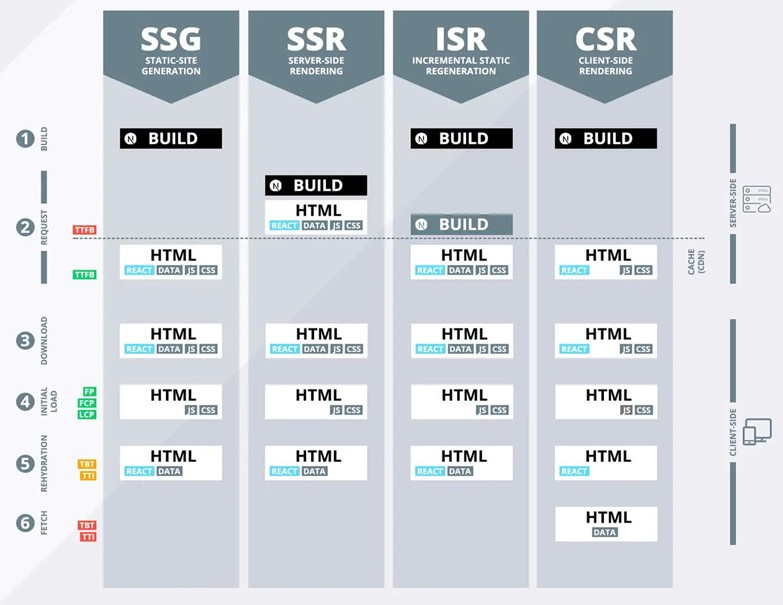
\includegraphics[width=\textwidth]{slike/uvod/pregled-strategija-iscrtavanja.jpg}
    \caption{Pregled strategija iscrtavanja u Next.js programskom okviru \cite{dumais2021nextjs}}
    \label{fig:pregled-strategija-iscrtavanja}
\end{figure}

% TODO Pregled programskih okvira ubaciti?